\documentclass{article}
\usepackage{main}

\title{Exercices : Représentation graphique de fonction}
\author{Seconde 9}
\date{3 Mars 2025}

\begin{document}
\maketitle
\begin{minipage}{0.45\textwidth}
    
    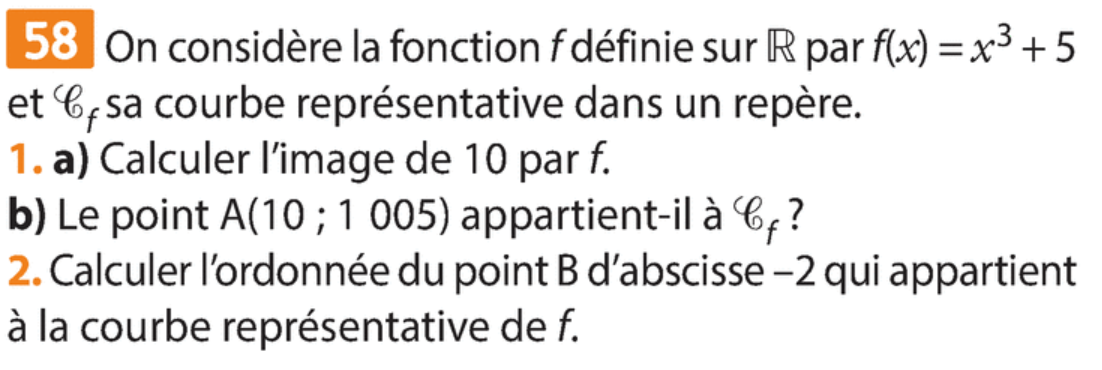
\includegraphics[width=\textwidth]{Exercice_1.png}
    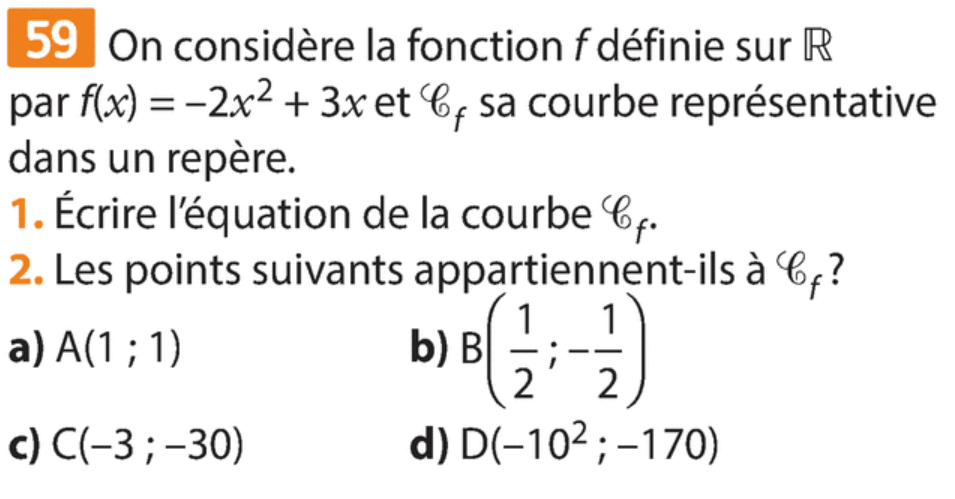
\includegraphics[width=\textwidth]{Exercice_2.png}
\end{minipage}
\hfill\vline\hfill
\begin{minipage}{0.45\textwidth}
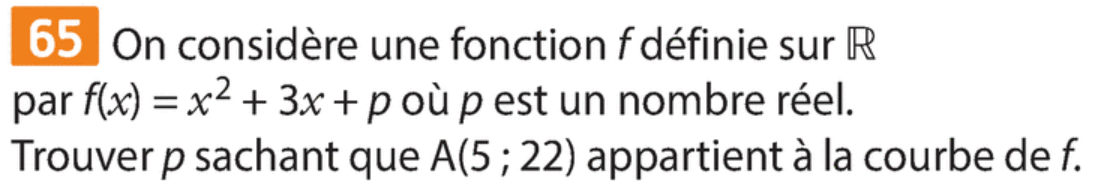
\includegraphics[width=\textwidth]{Exercice_3.png}
\end{minipage}

\vspace*{1cm}

\begin{minipage}{0.45\textwidth}
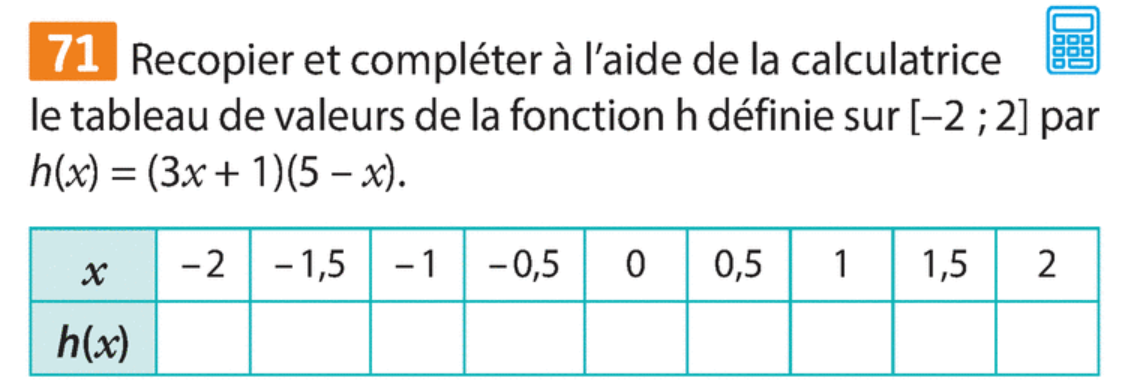
\includegraphics[width=\textwidth]{Exercice_4.png}
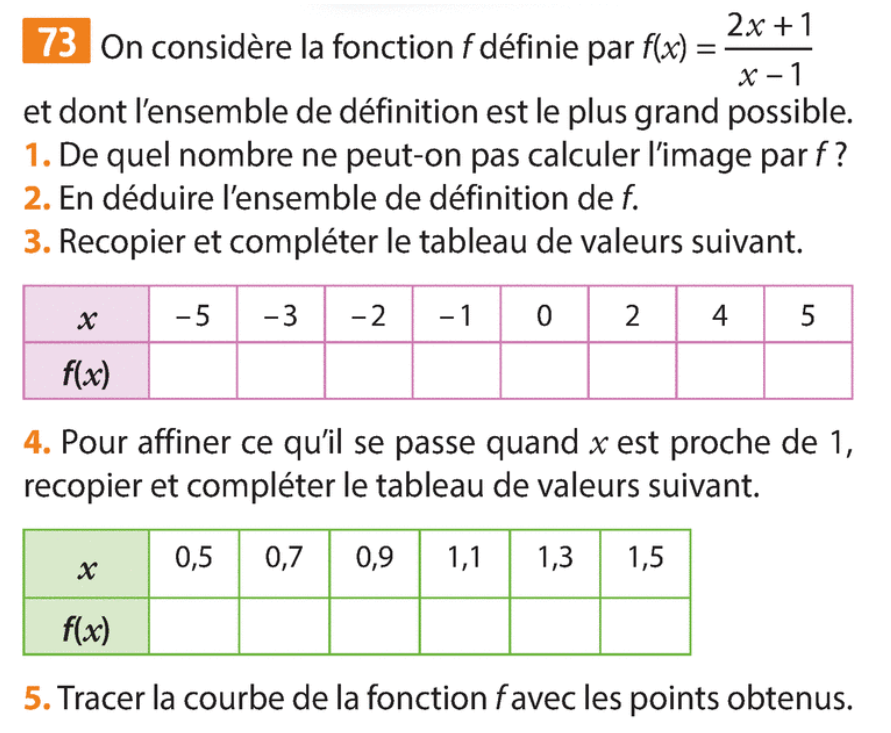
\includegraphics[width=\textwidth]{Exercice_5.png}
\end{minipage}
\hfill\vline\hfill
\begin{minipage}{0.45\textwidth}

\includegraphics[width=\textwidth]{Exercice_6.png}
\end{minipage}
\end{document}